% !TEX root = ../main.tex

\clearpage
\appendix

\section{Expanded Background}

\subsection{Prices}

If 1 BTC is worth \$3598.76 USD, as Google says it is at the time of writing, what does that actually mean? There are several subtleties here: (1) what that price actually represents, (2) the relationship between a quoted price and its actual price, (3) the concept that prices are really an exchange of one type of valuable good for another, and (4) the distinction between something's price and its value. The quoted price means that two (hopefully different\footnote{A trade between the same person is called a wash trade and is illegal in most regulated markets.}) people recently exchanged BTC and USD at a valuation of 1 BTC for \$3598.76 USD. First, note that it does not necessarily mean that exactly 1 BTC was exchanged --- it could have been 1 mBTC for \$3.60 or 1000 BTC for \$36M USD. Further, this valuation on the previous trade does not mean you will necessarily be able to exchange 1 BTC for \$3598.76 USD. Last sale price is an indicator of current price that becomes stale as time between subsequent exchanges increase (for example, for a house that last sold 30 years ago, last sale price on a house is not a good indicator of current price).

Instead, we will use the idea of that a cryptocurrency (or any asset) has two prices: (1) the most someone is willing to pay and (2) the least someone is willing to sell for. These are referred to as the best bid price and best ask (or offer) price respectively. Note that the best bid price should logically be less than the best ask price, otherwise an exchange would happen (such prices might occasionally `cross' but this should be temporal and quickly resolved with an exchange). The spread between these prices is called the bid-ask spread.

To understand why this is relevant to stablecoins, consider an example. Say a stablecoin is designed to ensure one unit is always priced at \$1 USD. To argue stability, one must show both that (1) the bid price should never exceed \$1 dollar and (2) the offer price should never dip below \$1 USD. Note, conversely, that bids can dip below \$1 USD (everyone prefers to pay less than something is worth) and asks can exceed \$1 USD (everyone prefers to receive more than something is worth).

\subsection{Exchange Rates}

Consider that several hours after writing the previous section, 1 BTC is now priced at \$3566.56 USD. In one sense, the price of BTC decreased by \$32.20. However it is exactly equivalent to say the price of \$1 USD increased by 0.002 mBTC. This raises a natural question: did BTC decrease in price or did USD increase in price? With an exchange rate, it is impossible to tell. We only know that the price of BTC and USD became closer in price over this short period of time.

To determine which currency is moving, one might consider a third or forth currencies (\cf US Dollar Index) to try and triangulate if BTC is moving in price, or USD is moving in price, or both. For example, in Figure~\ref{fig:btcandfiat} it certainly appears that BTC is the currency that is moving because the rest of the currencies are stable relative to each other. The only alternative is that USD, EUR, GBP, and CAD are volatile currencies that move together as a cluster relative to the stability of BTC. But it is much simpler to conclude that BTC is moving.

%========================%
\begin{figure*}[t]
	\centering
	\subfloat[GBP with respect to EUR and USD.]{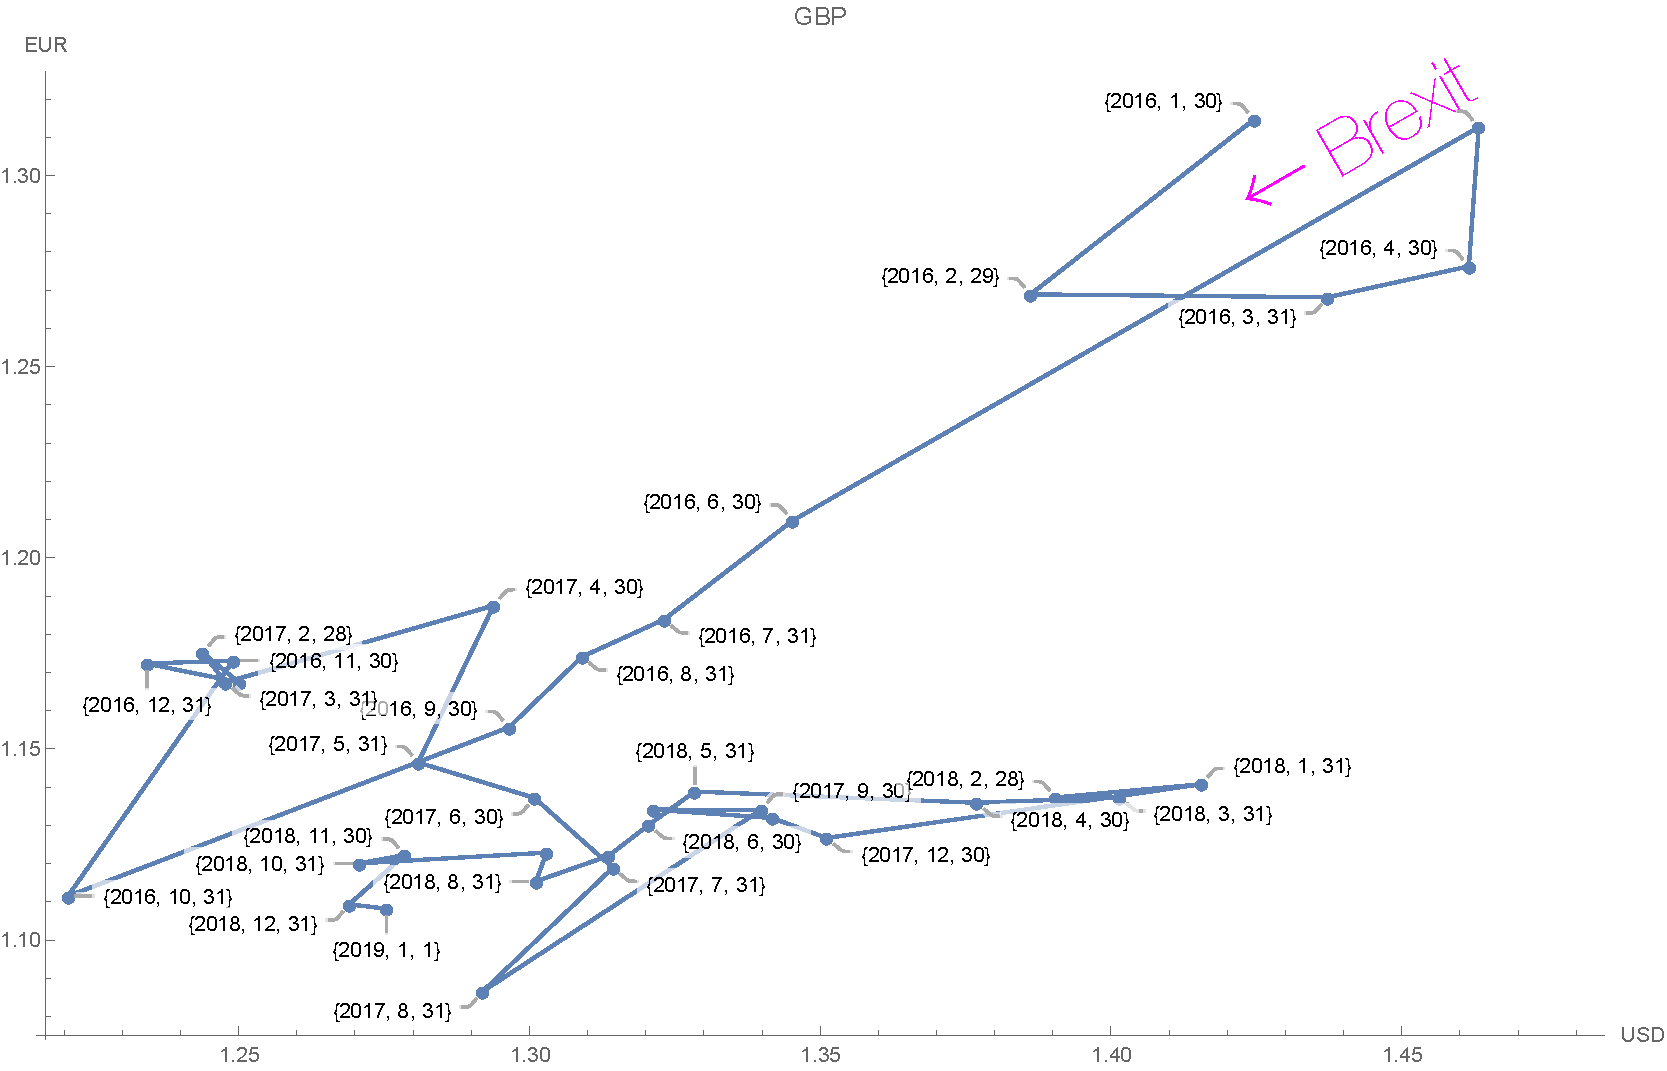
\includegraphics[width=0.65\textwidth]{figures/gbpBrexit.pdf}\label{fig:brexit}}
	\hfill
	\subfloat[Direction labels.]{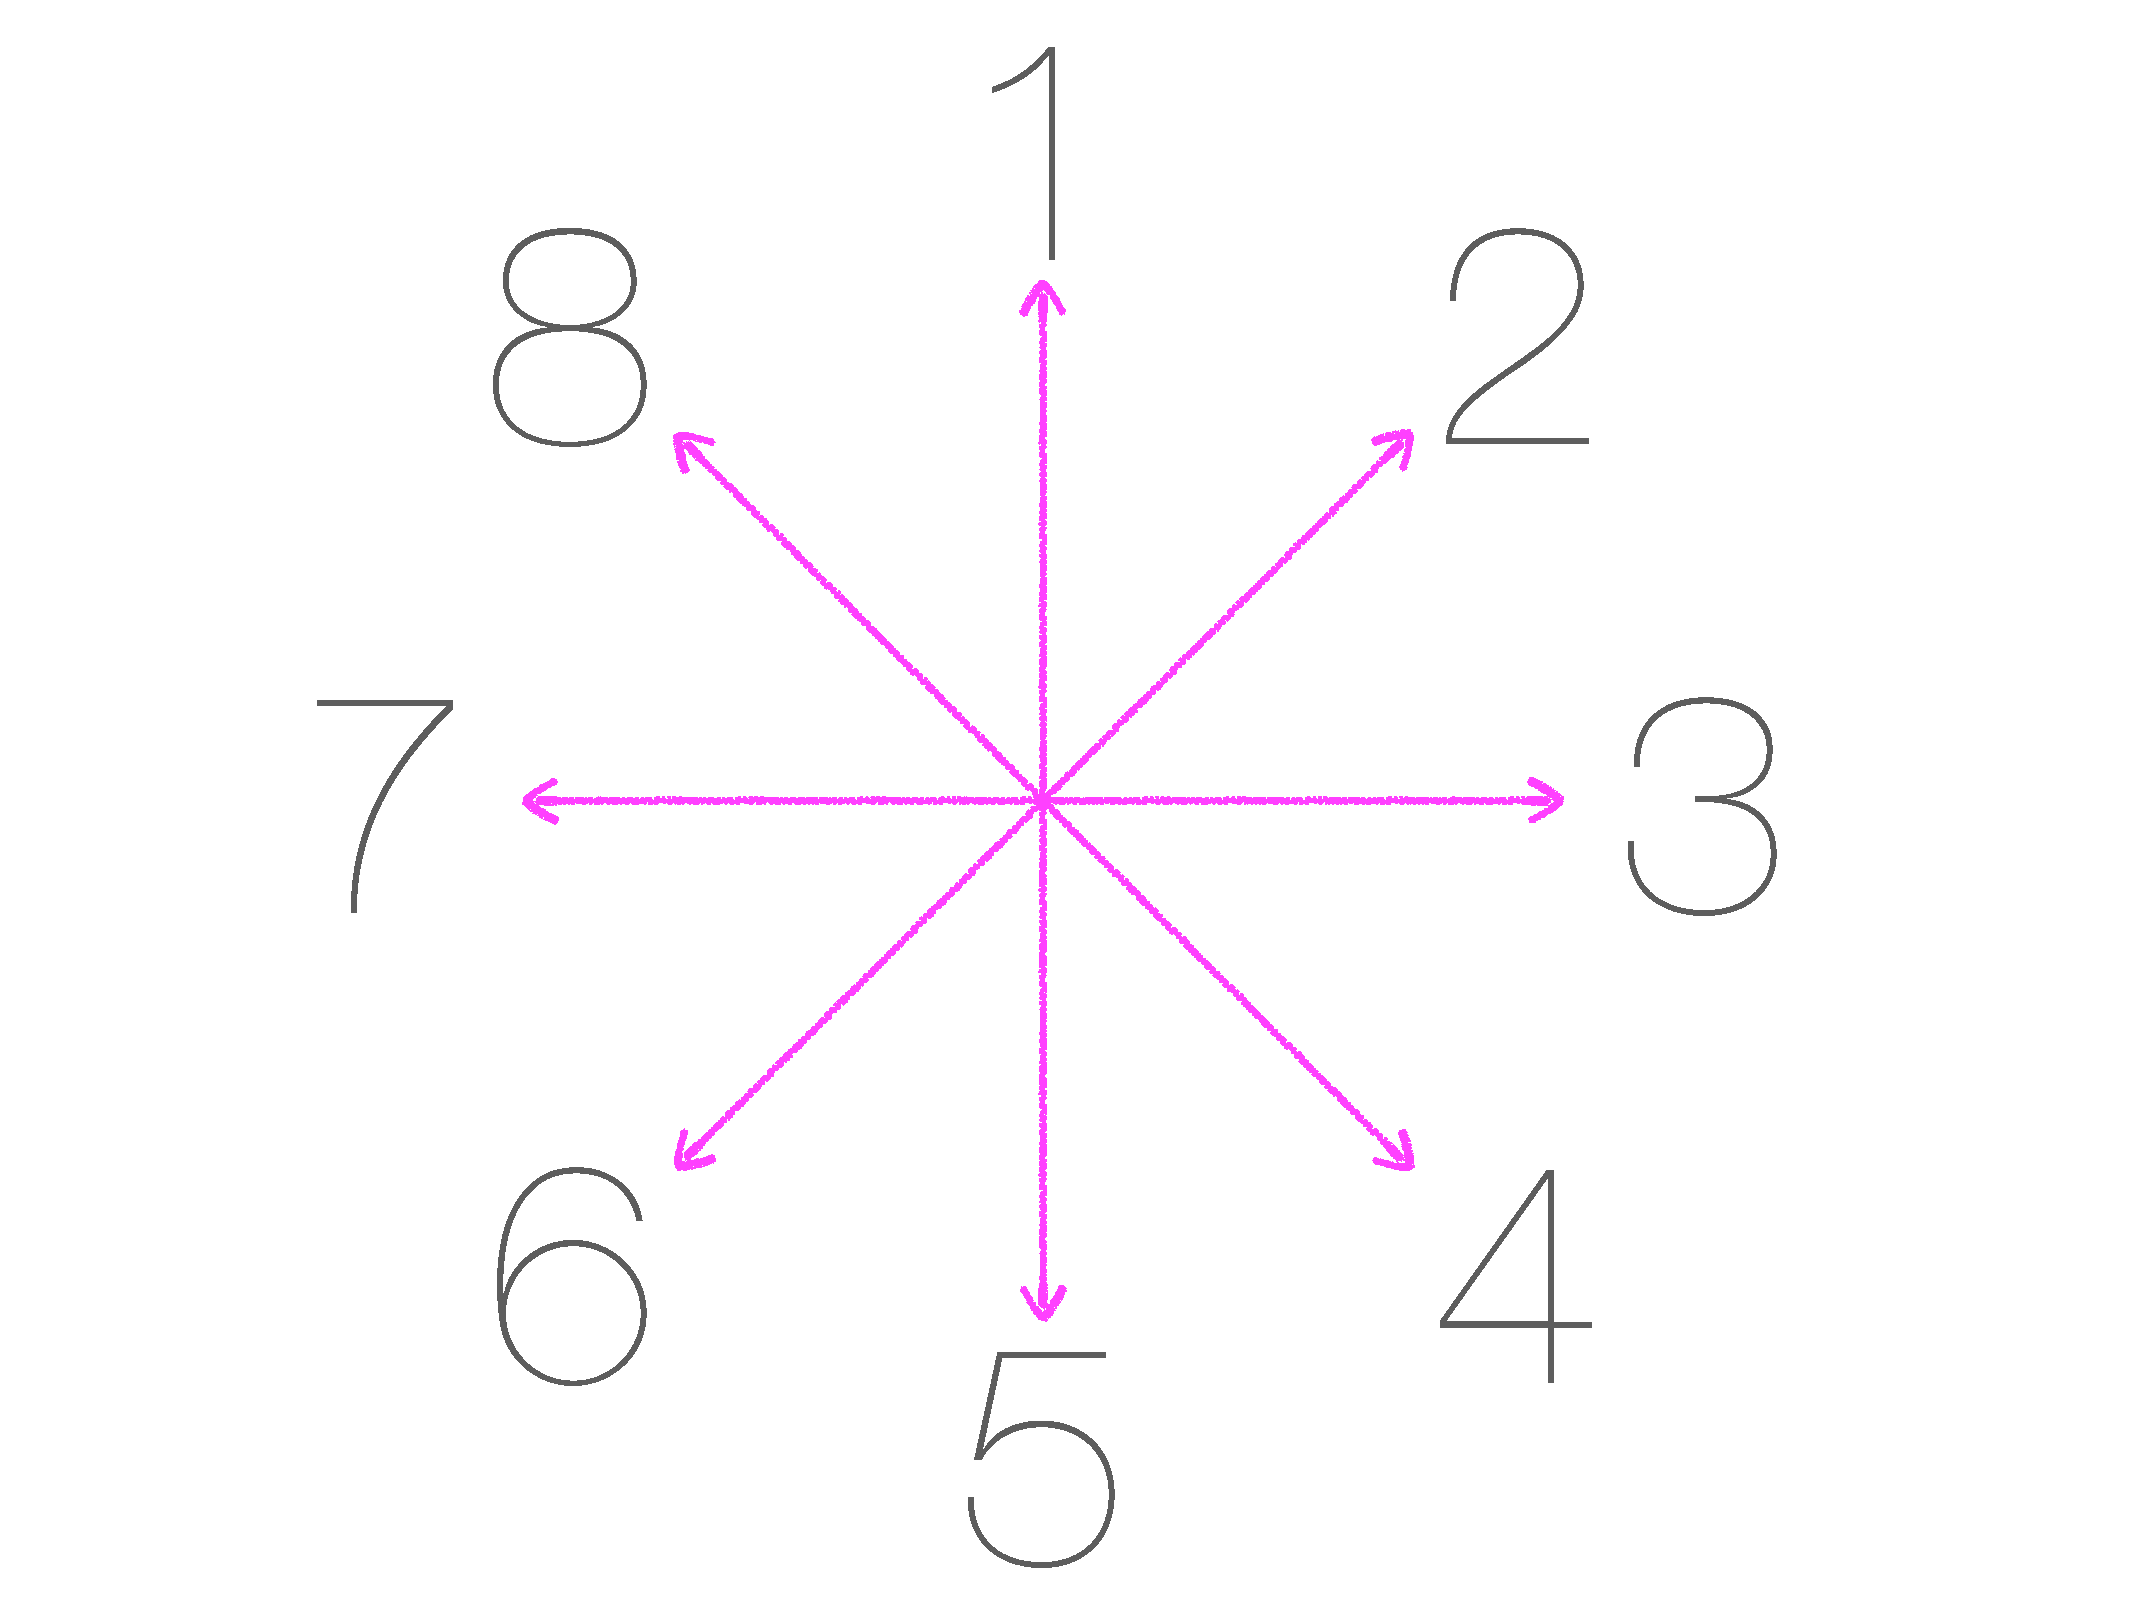
\includegraphics[width=0.25\textwidth]{figures/compass.pdf}\label{fig:legend}}
	\hfill
	\subfloat[The simpliest interpretation of the plots where $X$ refers to the currency on the x-axis (likewise $Y$).]{
	\begin{tabular}{|c|l|}
\hline
\textbf{Direction} & \textbf{Interpretation}   \\ \hline

         1/5                & $Y$ is losing (1) / gaining (5) value \\ \hline
         2/6                & Plotted asset is gaining (2) / losing (6) value \\ \hline
         3/7                & $X$ is losing (3) / gaining (7) value \\ \hline
         4/8                & \multicolumn{1}{p{13cm}|}{Plotted asset is gaining (4) / losing (8) value against $X$, while losing (4) / gaining (8) value against $Y$} \\ \hline

\end{tabular}
	}
	\caption{A connected scatter plot of GBP's exchange rate with EUR and USD demonstrating the effect of Brexit on GBP. Supporting documentation helps interpret the line movements in the plot.\label{fig:Comparison}}
\end{figure*}
%========================%

In order to apply this same logic in a visual way, we have created a number of charts like the one provided in Figure~\ref{fig:brexit}. Unlike most exchange rate graphs, these do not use a time axis. Instead each axis is a reference currency. In this case, the price of GBP (plotted value) in USD (x-axis) and EUR (y-axis) form a coordinate. For the last day of each month, a new coordinate is added and joined with a line from the previous value. This is inspired by similar charts on the website FiveThiryEight for things like kicking distance in football\footnote{``The 52 Best---And Weirdest---Charts We Made In 2016,'' \textit{FiveThirtyEight}, 30 Dec 2016.} and they have been called connected scatter plots.

Lines in a connected scatter plot can move in any direction. Figure~\ref{fig:legend} shows how we number the directions from 1 (upward or due north) clockwise to 8 (north-west). For each direction, we describe the simplest interpretation of what that price direction means. By simplest, we mean specifically that we keep an explanation that involves a single currency moving rather than an explanation that involves a pair of currencies moving in tandem. For example, in Figure~\ref{fig:brexit}, GBP shows a drastic movement along direction 6 starting at the time period marked Brexit. This means that GBP is losing value against both EUR and USD. The simplest explanation is that the movements are originating from GBP which is consistent with it losing value after Brexit. Later, GBP shows a lot of horizontal movements along the 7/3 line. The simplest explanation for this segment is volatility in USD rather than GBP.
A copy of the datasets and codes of all the charts can be found on our GitHub repository.\footnote{https://github.com/ Removed for anonymity.}

We will return to these charts later in Section~\ref{sec:stability} where we will use a government currency as one reference (USD on the x-axis) and a cryptocurrency as the other reference (BTC on the y-axis). A stablecoin should exhibit mostly vertical movements along the 1/5 direction.

\subsection{Valuation}

Recall that in the previous section, 1 BTC was priced at \$3566.56 USD. This means that two people recently swapped some amount of BTC and USD for the stated valuation. Does this mean 1 BTC is worth \$3566.56 USD? Value can mean different things in different contexts. The market value of a currency does present one type of value --- its replacement value, or the cost in USD to replace it. Note that more technically, one should  determine replacement value from the set of best offer prices sufficient to cover the volume of BTC being valued.

But does this mean that BTC is fundamentally worth \$3566.56 USD. This is unlikely because by the time you read this paper, the price of BTC in USD is probably quite different from this quoted value (perhaps humorously so). So what constitutes fundamental value? And why do prices change over time?

Stocks, which represent ownership in a firm, and thus a stake in the firm's equity. Therefore shares (called equities) have a fundamental value called its book value: simplified, it is the firm's capital or equity (the value of its assets minus the value of its liabilities, as reported on its annual audited financial statement) divided by the number of outstanding shares. Working in reverse, the price of a single share multiplied by the number of shares represents the market capitalization of the firm. In theory, these numbers should be the same but often are not. When the market capitalization exceeds the reported capital, the market believes the firm's capital will increase over time. If the market capitalization is less than the reported capital, it demonstrates a lack of confidence in the soundness of the firm's financial statements. Floating currencies like the USD, EUR, GBP, and CAD do not have the equivalent of a book value.

To explain Bitcoin's exchange rate with fiat currencies, an oft-repeated theory has emerged that attributes Bitcoin's value to the hydro consumed by blockchain mining. While imprecise, the theory suggests that if a valuable resource $x$ is consumed to produce $y$, the value of $x$ is imparted into $y$. Setting aside the nuance that the hydro contributed to the Bitcoin system only indirectly produces new coins (it produces blocks, and blocks produce coins only for now), there is no economic principle underlying this transfer of value.



\subsection{Stability and Volatility}

When the price of a currency changes over time, it is due to one of two reasons: new information about the currency's fundamental value (even if we cannot concretely say what it is) or transitory volatility due to the trading activites of uninformed traders~\cite{harris2003trading}. For a government issued currencies, information like national inflation rates, macro-economic policies, changes in trade flows, and changes in capital flows seem predictive of changes in the value of the country's currency~\cite{harris2003trading}. Note that a cryptocurrency, like Bitcoin, has none of these indicators. While volatility can be measured mathematically (using variances or deviations), most stablecoins do not offer a concrete, positive definition of what stability means. They tend to be defined by a negative sentiment of what they do not want (the volatility of Bitcoin) rather than a positive sentiment of what they do want.

\subsection{Functions of Money}

There is controversy over whether Bitcoin, and other cryptocurrencies, can even be classified as currencies. The original intent from Bitcoin's creator was for it to be a currency, however it has been assigned many different classifications: from a digitally scarce commodity, to a speculative instrument, to an entirely new asset class.

Most introductory finance textbooks classify currencies according to a set of three core properties they should fulfill for their users. it should operate as a medium of exchange, which roughly means that Alice will accept the currency from Bob because she is confident Carol will later accept it from her. Given the existence of exchange services, Bitcoin is generally considered an acceptable medium of exchange (albeit with some friction). Next, a currency is useful when it serves as the unit of account for pricing other assets. Bitcoin is almost never used as a unit of account and if goods are sold for Bitcoin, it is often priced in, say, USD with a short-lived (\eg 2 minute) spot conversion of the price to BTC for Bitcoin purchases. Finally, currencies should represent a stable store of value. Alice will not accept a currency that depreciates quickly in value from Bob because even though Carol might accept it, what she can obtain from Carol in exchange will be worth less. Less intuitively, currencies that appreciate quickly in value are equally problematic. Alice might gladly accept it from Bob but Bob is unlikely to part with it, and so currencies like this tend to be hoarded. They also hamper lending (see next section).

The goal of a stablecoin is to add the store of value feature to cryptocurrencies, which are already a somewhat adequate medium of exchange. Further, if the currency is stable, it may become a more prominent to use it as a unit of account. Thus stablecoins are intended to make cryptocurrencies more currency-like.~\cite{rogoff2017curse}

 %Cite Curse of Cash: Is its cited in the right place? (above parag)

\subsection{Lending}

Lending a volatile currency poses a risk for both the cash provider and cash taker. Currency depreciation results in the cash provider being repaid less than what they initially provided, and currency appreciation results in the cash taker having to repay a great amount than what was borrowed. Thus a stable currency enables low-risk lending which is beneficial to all participants and is the cornerstone of a modern economy. Okoye \etal put it in a way that is hard to improve on:

\begin{quote}

``It is difficult to overstate the role of lending in a modern economy. Take, as an illustrative example, the role of a central bank; one of the main national institutes (along with the treasury) that cryptocurrencies aim to displace. First and foremost, a central bank is an actual bank, providing accounts for its member banks to deposit money and earn interest. Member banks provide interest-earning accounts to the public. Interest is paid to the public because banks use the deposited money to form loans. Because central bank interest rates are low, banks prefer to lend to other banks any excess cash they hold at day's end instead of depositing them (other banks borrow to meet liquidity requirements). These loans earn interest, and central banks target this specific lending rate when they intervene in the economy. The most common intervention is the buying (circulating new money) or selling (removing circulating money) of government bonds, which are interest-earning loans from investors to the government. Central banks will also provide loans (of `last resort') to banks unable to secure loans from other banks, typically during some sort of liquidity crisis. An economy without loans would have no interest rates, no bonds, and essentially nothing for a modern central bank to do.~\cite{okoyetoward}''

\end{quote}

%========================%

\subsection{Bitcoin's Exchange Rate}

%Without government oversight, the exchange rate of Bitcoin is dependent on: (a) the supply and demand for exchanging Bitcoin and other things of value, namely fiat currencies such as the USD; (b) it's internal algorithm for releasing new BTC (Bitcoin's currency) on a fixed schedule; and (c) the market for participating in transaction validation which is integral into how new BTC comes into circulation.

% = = = = = = = = = = = = = = = = = = = = = = = = = = = = = = = = %

\section{Discussion Points}

Up to this point, we walked though our proposed taxonomy for stabilization techniques and described each mechanism in detail. In this section, we bring up some several important discussions on the stablecoin topic as we believe they make contributions to research on stablecoins. First, we provide an evaluation of stabilization mechanisms based on their trust assumptions and core idea. In the following we discuss oracles, used by some above techniques to obtain the exchange rate. Next, we elaborate on what stability means by visualizing it using a set of graphs. Finally, we explore and discuss the potential stable index-cryptocurrencies (namely Ethereum gas) in the context of stablecoins.

% = = = = = = = = = = = = = = = = = = = = = = = = = = = = = = = = %

\subsection{Evaluation of Stabilization Mechanisms}

We have considered various issues with different mechanisms of designing a stablecoin (discussed in Sections~\ref{sec:t1} and~\ref{sec:t2}). We provide a summary of these results in Table~\ref{tab:evframework} that evaluates each mechanism's core ideas and trust model. The columns and rows of the table are the evaluation criteria and mechanisms respectively. This framework provides a summary of the advantages and disadvantages of the different mechanisms for creating stablecoins.

%========================%

%\subsection{Why so many?}

%Emphasis on other things, like setting up contracts, governmence, audits, etc.
% Which blockchain

%========================%

\subsection{Oracles Everywhere}

A number of stablecoin proposals feature oracles which feed information about the stablecoin's exchange rate onto the blockchain. This is essential for indirectly-backed stablecoins, and incidental to intervention-based coins. This raises an important design question. A stablecoin exists so that a digital (or material) good or service can be effectively priced in, say, USD instead of in ETH. To be clear, it is priced in the stablecoin, which maintains a stable exchange rate with USD. To accomplish this, an oracle provides a reliable exchange rate and somewhat elaborates contracts issue stablecoins with an unusual risk profile (\eg full redemption might not be possible under certain market conditions) that could be difficult for non-experts to understand.

Let us take a step back and think about the larger picture. If we have trustworthy oracles providing reliable exchange rates, is it not a simpler design to just have transacting parties use the oracle directly? Anyone wanting to do business in a stable currency can determine at transaction time how much their good or service, priced in USD, is in ETH and charge the correct amount in ETH (which can then be immediately liquidated for USD, if desired). In summary, the oracle assumption that underlies many stablecoins is itself sufficient to side-step the need for stablecoins. This is applicable to lending as well: loans, interest rates, and repayment amounts can be denominated in USD but paid in ETH using a spot conversion via an oracle (\eg as proposed in~\cite{okoyetoward}).

%========================%

\subsection{Visualizing Stability}\label{sec:stability}

\begin{figure}[t!]
	\centering
	\subfloat[ETH]{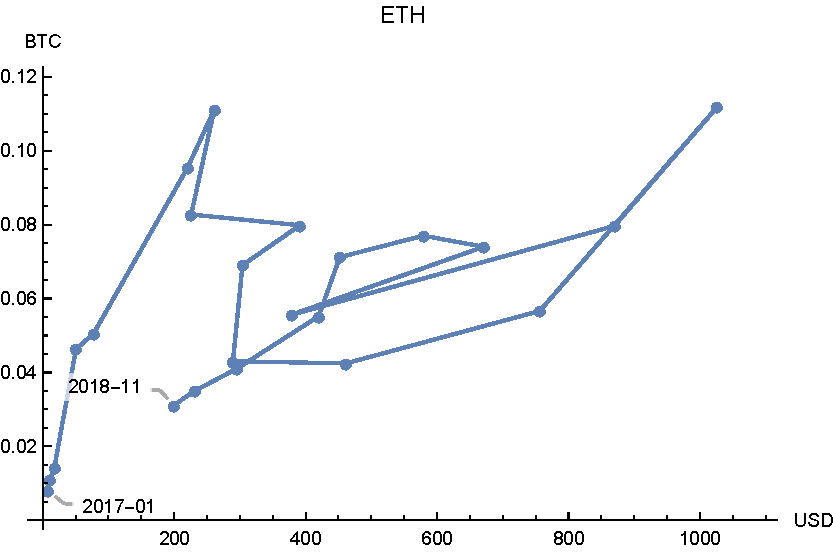
\includegraphics[width=0.45\textwidth]{figures/eth.pdf}\label{fig:eth}}
	\hfill
	\subfloat[XRP]{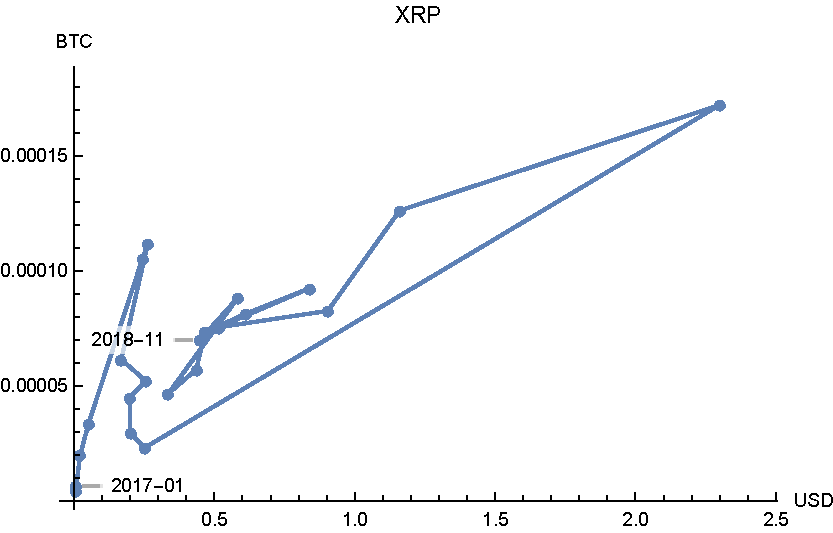
\includegraphics[width=0.49\textwidth]{figures/xrp.pdf}\label{fig:xrp}}
	\caption{Volatility in cryptocurrencies}
	\label{fig:fiatandcrypto}
\end{figure}

We show a connected scatter plot in Figure~\ref{fig:fiatandcrypto} that shows two cryptocurrencies, ETH and XRP (from Ripple) plotted against two reference currencies: the USD on the x-axis as a currency with government-managed stability, and Bitcoin which has no stability mechanism. Like Bitcoin, neither ETH nor XRP have a stability mechanism. The reader might anticipate one of two things: either (i) they move independently from the reference currencies (diagonal movements along the 2/6 direction) or (ii) they move in a way that is correlated to Bitcoin (3/7 movements) because the market prices all cryptocurrencies like a sector. From Figure~\ref{fig:fiatandcrypto}, it is fairly apparent that (i) is correct. The graph displays XRP's strong price surge in December 2017.


\begin{figure*}[t]
	\centering
	\subfloat[CAD]{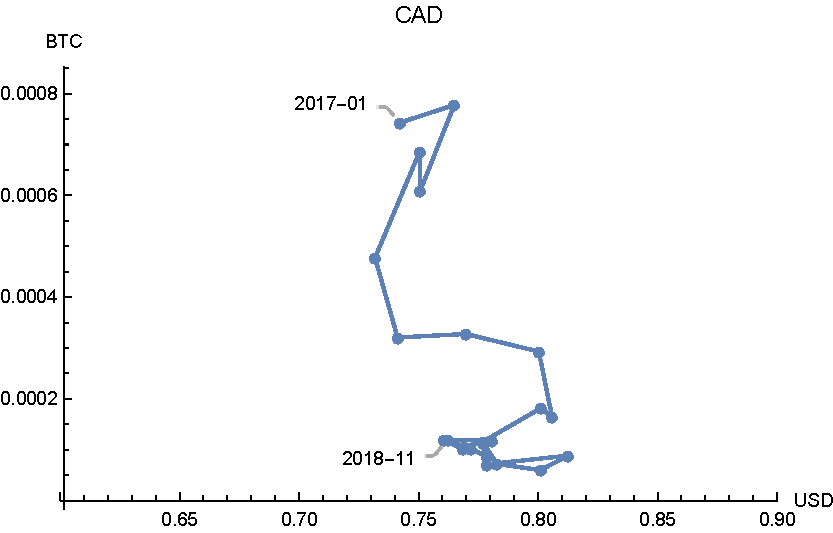
\includegraphics[width=0.45\textwidth]{figures/cad.pdf}\label{fig:cad}}
	\hfill
	\subfloat[EUR]{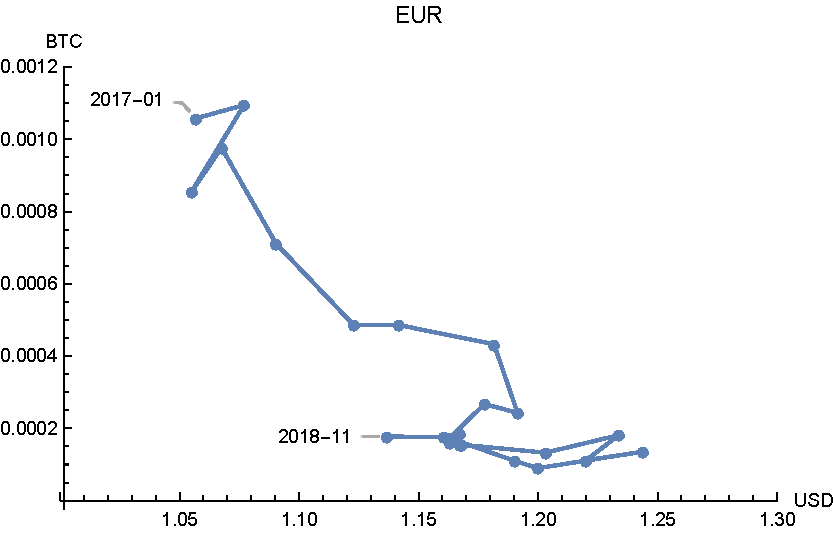
\includegraphics[width=0.45\textwidth]{figures/eur.pdf}\label{fig:eur}}
	\hfill
	\subfloat[Tether]{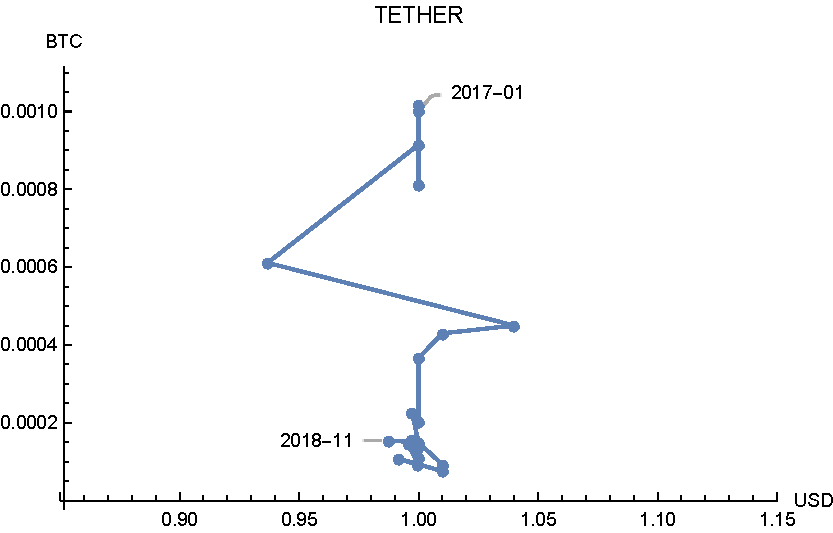
\includegraphics[width=0.45\textwidth]{figures/tether.pdf}\label{fig:tether}}
	\hfill
	\subfloat[BitUSD]{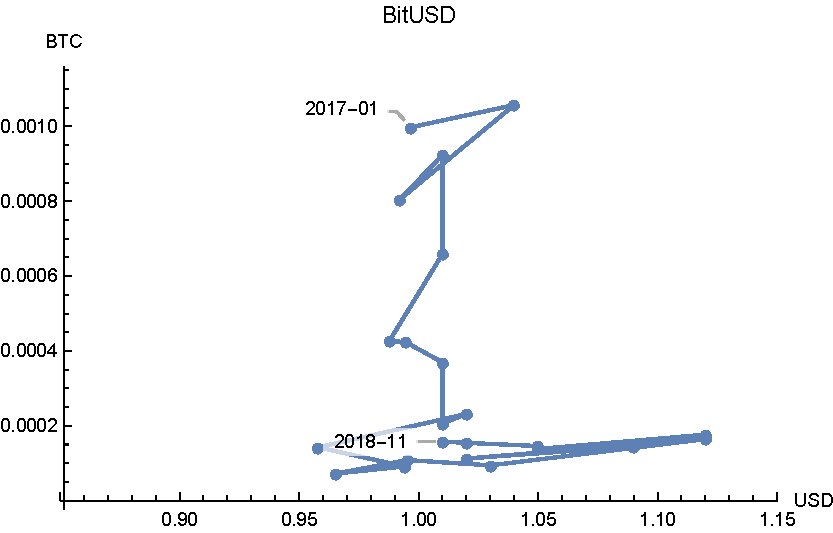
\includegraphics[width=0.45\textwidth]{figures/bitusd.pdf}\label{fig:bitusd}}
	\caption{Stability in two government-issued fiat currencies (CAD and EUR) and two stablecoin projects (Tether and BitUSD). Note that the x-axis is sized consistently across all four plots, with a \$0.30 USD spread. }
	\label{fig:all}
\end{figure*}

Next we plot a number of stablecoins in Figure~\ref{fig:all}. The top two plots are governmental currencies, the Canadian dollar and the Euro, which have no formal relationship to the USD but are managed by their central banks using similar policies and have intertwined economies. The bottom two currencies are two stablecoins, Tether (directly backed with USD) and BitUSD (indirectly backed with USD). All four currencies exhibit movements in 1/5 direction which indicate that most price movements are due to Bitcoin's volatility and not the volatility of either the plotted currency or USD. Note also that the spread of the x-axis is consistent across all four plots to allow cross-comparison. Both Tether and BitUSD exhibit some volatility. When Tether breaks from its stability with the USD, it moves in diagonal movements that are not correlated with either Bitcoin or USD. When BitUSD loses its stability relative to the USD, it moves in a horizontal 3/7 direction which is correlated with BTC.

%========================%

\subsection {Ethereum's gas: a stable `coin'?}\label{sec:GasInvs}

\begin{figure}[t]
	\centering
	\subfloat[Ethereum gas with respect to ETH and USD.]{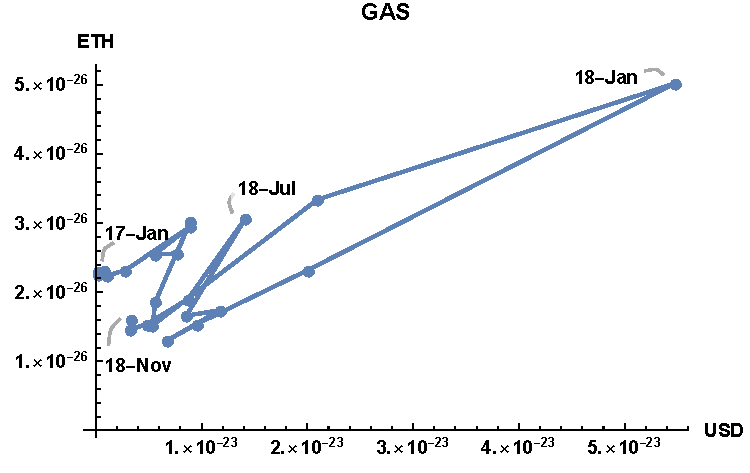
\includegraphics[width=0.49\textwidth]{figures/gasetherusd.pdf}\label{fig:gasetherusd}}
	\hfill
	\subfloat[Ethereum gas with respect to ETH and Electricity.]{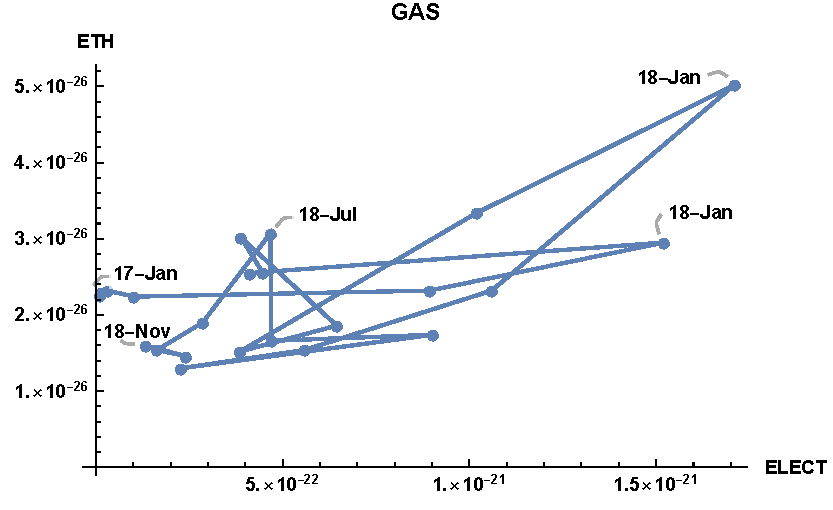
\includegraphics[width=0.49\textwidth]{figures/gaselectricityether.pdf}\label{fig:gaselectricityether}}
	\caption {Ethereum average gas price variations with respect to Ether, USD, and Electricity. As mentioned in the Section~\ref{sec:GasInvs}, the drastic movements in the charts represent specific events. Data is from January 2017 to November 2018.}
	\label{fig:gas}
\end{figure}

DApps on Ethereum execute arbitrary code provided by the owner of the DApp. While this code might be written in a high-level programming language like Solidity, it is compiled to a compact representation (called `bytecode') that is a set of low-level instructions to the environment (Ethereum virtual machine or EVM). Because different functions will have different complexities, the user running the function pays in proportion to the number of instructions, the complexity of the instructions, and the storage requirements. This means that each operation has a fixed price. Naturally the operations might be priced in ETH, since it is the on-board currency, however this would cause the price of computation to be as volatile as Ether itself. Instead, Ethereum uses a pseudo-currency called gas.\footnote{http://ethdocs.org/en/latest/contracts-and-transactions/account-types-gas-and-transactions.html\#what-is-gas} Each instruction has a fixed price in gas. A user who wants to run a function will offer to pay a certain amount of ETH per unit of gas to the miner who finalizes the function. Miners will generally choose which functions to run first based on how much ETH/gas they offer, and they might ignore functions that offer too little ETH/gas. We describe gas as a pseudo-currency because it cannot be directly stored or transacted, however we will revisit this below.

Gas was envisioned as maintaining a relatively stable value where a particular function should cost the same amount (say in USD) over time, even as the price of ETH changes dramatically (as seen in Figure~\ref{fig:eth}). We first investigate how successful gas has been with the charts in Figure~\ref{fig:gas}, which show the monthly average gas price variations with respect to USD and ETH in the first chart; and electricity and USD in the other. Electricity data is from a Canada-based average index which does not necessarily reflect the costs of mining on a global blockchain, like Ethereum, but if gas were correlated to electricity generally, it should be evident from a representative energy index. Gas demonstrates diagonal movements along the 2/6 direction meaning that it actually moves independently of ETH, USD and electricity. There is no strong evidence of stability. This could be due to a few factors. First, the graph is dominated by one large spike and one moderate spike which correspond to (i) when the popular Ethereum game Cryptokitties \footnote{Cryptokitties website \url{https://www.cryptokitties.co/}} was first launched (January 2018) and, (ii) when the China-based crypto exchange FCOIN \footnote{Fcoin website \url{https://www.fcoin.com}} was launched (July 2018) and required a lot of on-chain voting. Both these events  clogged up the Ethereum network and increased the gas price as users had to pay more gas for their transactions to go through. Second, it is probably true that users do not have a strong mental model of how much gas to stake for a computation and rely heavily on the user interface for prompts about gas.

Although gas might become a stable unit of account, it is not a store of value because it cannot be held or transacted. However gas could be used to back a stablecoin, much like the coins in the directly-backed category. Amazingly, such a gas-backed coin could even be made redeemable. Ethereum is designed in such a way that it allows users to create a smart contract which stockpiles and swaps gas with other tokens. Operations that store data on Ethereum blockchain modify its global state hence they are very expensive. So in order to incentivize users to free up space on the blockchain, Ethereum refunds the amount of gas users paid if they delete their smart contracts or stored data~\cite{wood2014ethereum}. GasToken is a directly-backed and redeemable tokenization of gas.\footnote{https://github.com/projectchicago/gastoken} When the gas price is low (\eg 1 Gwei), users can store some data on the GasToken contract and create GasTokens. Later when the gas price increases (\eg 50 Gwei), users can redeem their GasTokens. However they do not receive ETH back; rather, they use the tokens to pay the transaction fees for other computations. 

As users' mental model of gas improves over time, the volatility of gas has the potential to reduce. Gas-backed tokens represent a new class of stablecoin that float in value without any direct ties to USD, references to exchange rates, or explicit intervention mechanisms. It is an interesting subject worthy of further research. 

%========================%

%\subsection{Consequences for Central Banking}

%Interest rates: borrower pays her loan + interest
%Negative interest rate: borrower is paid the interest + she uses the loan
%Sweden and Japan are examples of countries that use NIR

%========================%

%\subsection{Liquidity Crisis and others}


%========================%

\section{Conclusion}

In this paper, we provide a survey of active stablecoin projects. Unlike previous research studies performed on this topic, we selectively use the concepts from finance while eliminating the jargons. In addition, rather than focusing on the details of how particular `brands' of stablecoins work, we thoroughly describe the fundamental mechanics and concepts to achieve price stability. Respectively, we show the taxonomy we use to classify stablecoins which represents the techniques to build a stablecoin. Additionally, we evaluate different price stability achieving mechanics based on their fundamental design decisions and trust models. The comparative evaluation framework highlights the advantages and disadvantages of each techniques more precisely. Eventually, we explore the potential stable index-cryptocurrencies (namely Ethereum gas) in the context of stablecoins.